\documentclass[conference]{IEEEtran}


\usepackage{cite}
\usepackage{pslatex} % -- times instead of computer modern, especially for the plain article class
\usepackage[colorlinks=false,bookmarks=false]{hyperref}
\usepackage{booktabs}
\usepackage{graphicx}
\usepackage{xcolor}
\usepackage{multirow}
\usepackage{comment}
\usepackage{listings}
%\usepackage{flushend} % even out the last page, but use only at the end when there is a bibliography
%\usepackage{minted}		% For inserting code
%\setminted[systemverilog]{
%	tabsize=3
%}
%\setminted[C]{
%	tabsize=3,
%	breaklines
%}
%\setminted[scala]{
%	tabsize=3,
%	breaklines
%}
\usepackage{xspace}		% For using \SV with trailing spaces
\usepackage{cleveref}	% Needed for correctly referencing listings
\usepackage{subfig}

\newcommand{\code}[1]{{\small{\texttt{#1}}}}
\newcommand{\SV}{SystemVerilog\xspace}


% fatter TT font
\renewcommand*\ttdefault{txtt}
% another TT, suggested by Alex
% \usepackage{inconsolata}
% \usepackage[T1]{fontenc} % needed as well?

%\newcommand{\todo}[1]{{\emph{TODO: #1}}}
\newcommand{\todo}[1]{{\color{olive} TODO: #1}}
\newcommand{\martin}[1]{{\color{blue} Martin: #1}}
\newcommand{\simon}[1]{{\color{green} Simon: #1}}
\newcommand{\abcdef}[1]{{\color{red} Author2: #1}}
\newcommand{\rewrite}[1]{{\color{red} rewrite: #1}}
\newcommand{\ducky}[1]{{\color{orange} Richard: #1}}
\newcommand{\kasper}[1]{{\color{purple} Kasper: #1}}
\newcommand{\hjd}[1]{{\color{pink} Hans: #1}}

% uncomment following for final submission
%\renewcommand{\todo}[1]{}
%\renewcommand{\martin}[1]{}
%\renewcommand{\simon}[1]{}
%\renewcommand{\kasper}[1]{}
%\renewcommand{\ducky}[1]{}



%%% ZF
\usepackage{listings}
\lstset{
	columns=fullflexible,
	%        basicstyle=\ttfamily\footnotesize,
	basicstyle=\ttfamily\small,      
	%columns=fullflexible, keepspaces=true,
	numbers=left,    
	numberblanklines=false,
	captionpos=b,
	%	breaklines=true,
	escapeinside={@}{@},
	numbersep=5pt,
	language=C,
	tabsize=2,
	breakatwhitespace=true,
	breaklines=true,
	deletekeywords={for},
	%        keywordstyle=\ttfamily
	numbersep=5pt,
	xleftmargin=.10in,
	%xrightmargin=.25in
}

\newcommand{\longlist}[3]{{\lstinputlisting[float, caption={#2}, label={#3}, frame=tb, captionpos=b]{#1}}}

\title{ChiselVerify: An Open-Source Verification Method with
Chisel and Scala}

\author{\IEEEauthorblockN{Andrew Dobis, Tjark Petersen, Kasper Juul Hesse Rasmussen, Enrico Tolotto, \\
Hans Jakob Damsgaard, Simon Thye Andersen, Richard Lin, Martin Schoeberl}\\
\IEEEauthorblockA{\textit{Department of Applied Mathematics and Computer Science} \\
\textit{Technical University of Denmark}\\
Lyngby, Denmark \\\\
\textit{Department of Electrical Engineering and Computer Sciences} \\
\textit{UC Berkeley}\\
Berkeley, CA \\\\
andrew.dobis@alumni.epfl.ch, s186083@student.dtu.dk, s183735@student.dtu.dk, s190057@student.dtu.dk, \\
s163915@student.dtu.dk, simon.thye@gmail.com, richard.lin@berkeley.edu, masca@dtu.dk}
}

%\author{\IEEEauthorblockNAndrew Dobis, Tjark Petersen, Kasper Juul Hesse Rasmussen, Enrico Tolotto, \\
%Hans Jakob Damsgaard, Simon Thye Andersen, Richard Lin, Martin Schoeberl}\\
%\IEEEauthorblockA{\textit{Department of Applied Mathematics and Computer Science} \\
%\textit{Technical University of Denmark}\\
%Lyngby, Denmark \\\\
%\textit{Department of Electrical Engineering and Computer Sciences} \\
%\textit{UC Berkeley}\\
%Berkeley, CA \\\\
%andrew.dobis@alumni.epfl.ch, s186083@student.dtu.dk, s183735@student.dtu.dk, s190057@student.dtu.dk, \\
%s163915@student.dtu.dk, simon.thye@gmail.com, richard.lin@berkeley.edu, masca@dtu.dk}
%}


\begin{document}

\maketitle \thispagestyle{empty}


\begin{abstract}
Performance increase with general-purpose processors has come to a halt.
We can no longer depend on Moore's Law to increase computing performance.
The only way to achieve higher performance or lower energy consumption
is by building domain-specific hardware accelerators.
To efficiently design and verify those domain-specific accelerators, we need
agile hardware development. One of the main obstacles when proposing such a modern method
is the lack of modern tools to attack it. To be able to verify a design in such a time-constrained development
method, one needs to have efficient tools both for design and verification.

This paper thus proposes ChiselVerify, an open-source tool for verifying
circuits described in Chisel. It builds on top of the Chisel
hardware construction language and uses Scala to drive the verification process.
ChiselVerify is created based on three key ideas.
First, our solution highly increases the productivity of the verification engineer, by allowing hardware testing to be done in a modern high-level programming environment.
\hjd{This needs covering later in the paper.} Second, the framework functions with any hardware description language thanks to the flexibility of Chisel blackboxes.
Finally, the solution is well integrated into the existing Chisel universe, making it an extension of currently existing testing libraries.

%We implement ChiselVerify in a way inspired by the functionalities found in SystemVerilog. This allows one to use
%functional coverage, constrained-random verification, bus functional models, transaction-level modelling and much more
%during the verification process of a design in a contemporary high-level programming ecosystem.
\end{abstract}

\begin{IEEEkeywords}
digital design, verification, Chisel, Scala
\end{IEEEkeywords}

\section{TODO}

\begin{itemize}
\item incorporate the reviews
\item add \url{http://people.eecs.berkeley.edu/~ksen/papers/rfuzz.pdf} to related work
\item Find a new venue abstract May 28: \url{http://www.iccd-conf.com/Home.html|}
\item \hjd{Do we write Scala package names in italic or not? \textit{ChiselTest} seems to be most common, so I have corrected some places.}
\item \hjd{Perhaps the use case is a bit too lengthy... Implementation details are not interesting here; the testing is, and it takes up little of the section.}
\end{itemize}


%\begin{verbatim}
%Dear Martin Schoeberl:
%
%I am sorry to inform you that the following submission was not selected by the program committee to appear at SAMOS XXI 2021:
%
%ChiselVerify: An Open-Source Verification Method with Chisel and Scala
%
%The selection process was very competitive. Due to time and space limitations, we could only choose a small number of the submitted papers to appear on the program. Nonetheless, I still hope you can attend the conference.
%
%I have enclosed the reviewer comments for your perusal.
%
%Best Regards, 
%Matthias Jung, PC SAMOS XXI
%
%============================================================================ 
%SAMOS XXI 2021 Reviews for Submission \#33
%============================================================================ 
%
%Title: ChiselVerify: An Open-Source Verification Method with Chisel and Scala
%Authors: Andrew Dobis, Tjark Petersen, Kasper Hesse, Enrico Tolotto, Hans Damsgaard, Simon Andersen, Richard Lin and Martin Schoeberl
%
%
%============================================================================
%                            REVIEWER \#1
%============================================================================
%
%---------------------------------------------------------------------------
%Reviewer's Scores
%---------------------------------------------------------------------------
%Evaluation of the work and contributions (1-5): 3
%           Originality and Novelty (1-4): 3
%                         Relevance (1-5): 5
%            Overall Recommendation (1-4): 2
%                        Best Paper Award: No
%                  Your Familiarity (1-3): 3
%
%Detailed Comments
%---------------------------------------------------------------------------
%The paper presents ChiselVerify, an open source framework for verification of circuits modeled in Chisel. Chisel is a framework developed previously in other works. ChiselVerify appears to be based on ChiselTest, a previously developed testing framework for Chisel. ChiselVerify appears to extend ChiselTest with constraint based coverage.
%
%The paper definitely presents a valid contribution and ChiselVerify should be a very useful verification environment for Chisel. Unfortunately, the paper is badly written, with little structure to help the reader understand the contributions and navigate the different sections. Even basic questions, such as what exactly is ChiselVerify? what inputs does it take? what outputs does it produce? how is it implemented? what other software does it use? etc. are left untouched.
%
%As it stands, the paper reads more like a juxtaposition of different sections written by various people, with no connection to one another. I believe that a significant rewrite is necessary before publication.
%
%Ira. D. Baxter -> Ira D. Baxter
%---------------------------------------------------------------------------
%
%
%
%============================================================================
%                            REVIEWER \#2
%============================================================================
%
%---------------------------------------------------------------------------
%Reviewer's Scores
%---------------------------------------------------------------------------
%Evaluation of the work and contributions (1-5): 3
%           Originality and Novelty (1-4): 2
%                         Relevance (1-5): 3
%            Overall Recommendation (1-4): 2
%                        Best Paper Award: No
%                  Your Familiarity (1-3): 3
%
%Detailed Comments
%---------------------------------------------------------------------------
%This paper proposes ChiselVerify, an open-source tool for verifying circuits described in Chisel. The idea is both good and timely. However, I could not get a clear picture of what is ChiselVerify, and what are its strengths and weaknesses. Does it support testing FSMs? Possibly as the test example shows some, but how? This paper is an extension of [15]. How does it differ from that work? The authors claim the main contribution of this paper is ChiselVerify, an open-source verification library for hardware designs. As such I would expect the paper to focus on the description of the tool and its functionality.
%
%A section named "Verification of AXI4 Interfaced Components" is offered, and mentions "bus functional models" (BFMs). However it is unclear if any BFM is supported and what is the required effort to produce/include them
%
%Treadle: cite this work. This section appears interesting but it not a contribution of this paper
%
%A sorting hardware use case is described, but actual testing text consists of two parahgraphs 
%
%Overall which ether topic is interesting, the presentation lacks focus.
%---------------------------------------------------------------------------
%
%
%
%============================================================================
%                            REVIEWER \#3
%============================================================================
%
%---------------------------------------------------------------------------
%Reviewer's Scores
%---------------------------------------------------------------------------
%Evaluation of the work and contributions (1-5): 4
%           Originality and Novelty (1-4): 3
%                         Relevance (1-5): 4
%            Overall Recommendation (1-4): 3
%                        Best Paper Award: No
%                  Your Familiarity (1-3): 2
%
%Detailed Comments
%---------------------------------------------------------------------------
%This paper presents ChiselVerify, an open-source tool for verifying circuits described in Chisel. It builds on top of the Chisel language and uses Scala to drive the verification process, thus the effectiveness (productivity) of verification phases can be improved. 
%In general, the paper is easy to read and follow. The fact that the author released it as open source is well received. 
%The paper is useful to verification engineers.
%---------------------------------------------------------------------------
%
%
%
%============================================================================
%                            REVIEWER \#4
%============================================================================
%
%---------------------------------------------------------------------------
%Reviewer's Scores
%---------------------------------------------------------------------------
%Evaluation of the work and contributions (1-5): 4
%           Originality and Novelty (1-4): 2
%                         Relevance (1-5): 4
%            Overall Recommendation (1-4): 3
%                        Best Paper Award: No
%                  Your Familiarity (1-3): 2
%
%Detailed Comments
%---------------------------------------------------------------------------
%In this work, ChiselVerify, an open-source tool for verifying circuits described in Chisel, is proposed.It builds on top of the Chisel hardware construction language and uses Scala to drive the verification process.
%The manuscript is very well organized and written presenting thoroughly all the steps of the research. The target problem and its importance are presented and discussed in detail as well as the previous work. Also, the proposed design methodology are presented in a clear and detailed way. All the sections of the paper balance very effectively between the background information of each topic and the explanation of each implementation. Moreover, both the examples throughout the sections and the final example, it seems the ideal way to make a reader have a deep understanding of this work. Finally the fact that this work is in open source, underlines and emphasizes the reliability of this work. 
%However an interesting information would be a comparison of this kind of verification(that this work proposes) compared to more conservatives methods in relation to time needed for each method, and effectiveness.
%---------------------------------------------------------------------------
%
%
%-- 
%SAMOS XXI 2021 - https://www.softconf.com/l/samos-xxi
%\end{verbatim}


\section{Introduction}
\label{sec:introduction}

We can no longer depend on Moore's Law to increase computing performance~\cite{dark-silicon:2011}.
Performance increase with general-purpose processors has come to a halt.
The only way to achieve higher performance or lower energy consumption
is by building domain-specific hardware accelerators~\cite{domain-hw-acc:2020}.
These accelerators can be built in chips or in FPGAs in the cloud.
%The production of a chip is costly. Therefore, it is essential to get
%the design right at the first tape-out. Thorough testing and verification of the design is mandatory.

To efficiently develop and verify those accelerators, we can learn from software development trends such as agile software development~\cite{agile:manifesto}.
We believe that we need to adapt to agile hardware development~\cite{henn-patt:turing:2019}.

Furthermore, as accelerators become part of the cloud service, i.e., FPGAs in the cloud,
software developers will increasingly need to adapt critical algorithms to FPGAs to enhance performance.
Hence, it is imperative to make accelerator design accessible for software developers.
By adapting hardware accelerator design to the methods and tools of contemporary software design,
it is possible to bridge both domains catering for a more uniform hardware/software development process.

Up until a few years ago, the two main design languages, Verilog and VHDL, dominated the
design and testing of digital circuits.
%However, both languages are decades behind
%modern languages for software development.
However, compared to software development and testing, digital design and testing methods/tools 
lack several decades of development. We propose a tool that
leverages software development and testing methods for digital design.
Based in the hardware construction language Chisel~\cite{chisel:dac2012}, which itself is embedded in Scala,
our framework reimagines functionalities form Universal Verification Method (UVM) with SystemVerilog~\cite{SystemVerilog} and
adapts them for the existing Chisel ecosystem.

We thus developed a method and concrete tools for agile hardware development.
ChiselVerify combines tools, languages, development, and testing methods from the last decades in
software development and applies them to hardware design.
We aim to raise the tooling level for a digital design to increase productivity.
The workload demanded for the verification (testing) of digital systems is about double the time of developing
them in the first place.

%Using the power and flexibility of Chisel Blackboxes, our tool can be used to verify
%designs implemented in any of the major hardware description languages (i.e., VHDL or Verilog)
%with little overhead. Furthermore, golden models described in any programming language can be
%used using the Java JNI. Our work builds upon existing open-source projects and 
%is thus also open-source.

We developed an object-oriented and functional framework for verification in Scala.
This framework is inspired by UVM, but leverages Scala's conciseness with the
combination of object-oriented programming with functional programming.
An initial experiment of testing the accumulator circuit of the Leros processor~\cite{leros:arcs2019}
showed the that a test written with UVM was about 800 lines of code, where a Scala based
test was around 80 lines of code~\cite{verify:chisel:2020}.
However, UVM supports more functionality that a plain ChiselTest in Scala.

%Within our verification framework, we support mixed language verification.
%Verilog can easily be combined with Chisel, as Chisel generates Verilog, and
%we use ChiselTest as a driver for the open-source Verilog simulator Verlator.
%With Yosys synthesis suite~\cite{Yosys} and GHDL~\cite{ghdl}
%we can translate VHDL into Verilog.
%
%A verification method is only usable when it can handle mixed-source designs.
%This means a Scala driven method must be able to test components written in Verilog,
%VHDL, and SystemVerilog.
%
%Chisel has support for black boxes, which allows the use of Verilog code within the Chisel design.
%Therefore, it is relatively easy to integrate Verilog components when wrapped into a black box.
%However, this forces Chisel to use Verilator instead of Treadle to run the simulation, impacting
%startup time.
%
%Chisel does not fully support VHDL. It can support VHDL using VCS, but there is no
%open-source solution available for VHDL simulation. For companies with a lot of source code written in VHDL this is a concern, as they must be able to integrate their existing IP in a Scala/Chisel based design and verification workflow.
%All major commercial simulation and synthesis tools support mixed-language designs, but no open-source tools exist that provide the same functionality.


This paper is an extension of \cite{verify:chisel:2020}.

\todo{What is different from the workshop paper}. Then main contributions of
this paper is ChiselVerify, an open-source verification library for hardware designs.

\todo{Rewrite section order}
The paper is organized in 7 sections.
Section 2 describes background and related work.
Section 3 describes our addition of constraint random verification to Chisel.
Section 4 gives an example of a bus functional model in Chisel for AXI.
Section 5 describes our addition of coverage to Chisel tests.
Section 6 explores ChiselVerify on a use case from industry.
Section 7 concludes.


\section{Background on Verification}
\label{sec:background}

This section will present a brief overview of what hardware verification is. We will also talk about Chisel, as well as the current solutions that exist in it with regards to the verification of digital systems.

\subsection{Verification of digital designs}
Verification of digital systems refers to the testing of a design before it has been taped-out~\cite{spear2008systemverilog}. This is in contrast to validation, which refers to testing a taped-out version of a digital circuit. 
It is difficult to talk about the verification of digital designs without mentioning SystemVerilog~\cite{SystemVerilog}, which is one of the main languages used for verification.
This is due to the wide variety of verification-centric functionalities that the language offers, which focus on improving the efficiency of writing test-benches rather than the testing itself.
SystemVerilog is an extension of Verilog, adding verification features and object-oriented programming to the mix. 
The language enables verification engineers to define constraint-driven randomized test-benches as well as define metrics to gather functional coverage data related to a test-suite. 
However, the verification functionalities are quite limited and trapped in a complex low-level language. 
SystemVerilog does however prove itself to be a good inspiration for the development of a high-level verification framework, which is what we did with ChiselVerify.

\subsection{Digital Design with Chisel}
In order to understand the context of our work, one first needs to know about the environment we are working in.
Chisel is a ``Hardware Construction Language'' embedded in Scala, used to describe digital circuits~\cite{chisel:dac2012}.
This language is much more high-level than the traditional hardware description languages, such as VHDL or Verilog, and allows for object-oriented and functional programming in the context of digital design.
One of the main aspects of Chisel that makes it so compelling is its full integration in the Java/Scala ecosystem.

Indeed, since Chisel and Scala are executing on the Java virtual machine, they have a very good interoperability with Java. 
We can therefore leverage a large pool of Java and Scala libraries for hardware design and verification. 
Furthermore, the name space of packets in Scala/Java simplifies integration of external components.
Open source hardware components in Chisel can thus be organized in the same manner as software libraries in Maven servers.

Working in the JVM also allows for the use of the Java JNI (Java Native Interface), which enables JVM based languages to call C functions and use their functionality.
This makes it possible to have co-simulations between Scala/Chisel testers and a C-based golden model. 
Ideally, this should allow companies to keep their existing C models, but move their simulation workflow into Scala/Chisel testers.

Another important thing to note is that Chisel is solely a hardware \emph{construction} language, and thus all valid Chisel code maps to synthesizable hardware.
By separating the hardware construction and hardware verification languages, it thus becomes impossible to write non-synthesizable hardware and, in turn, speeds up the design process.

To go more into detail about how Chisel works, it starts by being translated into an intermediate representation called FIRRTL~\cite{firrtl}. It then goes through multiple optimization stages, called \textit{Transforms}, during which high-level concepts, such as a functional \texttt{map} or vectors, are compiled into lower level concepts that map nicely onto what we normally see in a Verilog or VHDL description. Once that is done, the newly transformed FIRRTL, called Low FIRRTL, can be used either for simulation, using an execution engine such as Treadle, or for synthesis by translating it into Verilog which is then used to generate the synthesised circuit. Note that the final Verilog description may also be used for simulation purposes using engines such as verilator~\cite{verilator}. An overview of the Chisel pipeline can be found in figure \ref{fig:chisel-pipe}.

\begin{figure}
    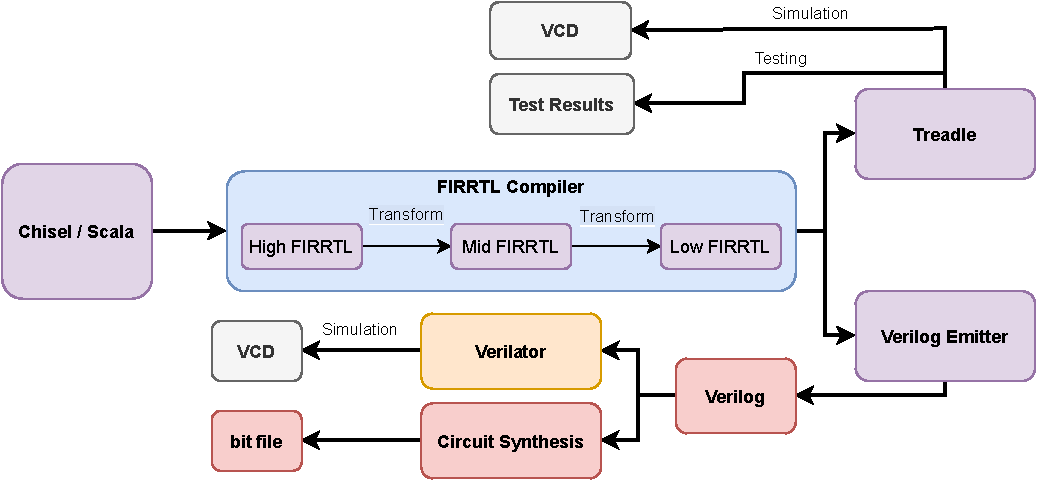
\includegraphics[width=9cm]{Chisel_FIRRTL_VERILOG.pdf}
    \caption{Overview of the Chisel pipeline.}
\label{fig:chisel-pipe}
\end{figure}

All of these things make Chisel feel much more contemporary than its predecessors.

\subsection{Testing Chisel Designs}
An aspect that can't be omitted from any Hardware Construction Language, is a way to test systems built in it.
A digital design described in Chisel can be tested with ChiselTest~\cite{chisel:tester2}, a non-synthesizable testing framework for Chisel.
ChiselTest emphasizes on usability and simplicity while providing ways to scale up in complexity.
Fundamentally, ChiselTest is a Scala library that provides access into the simulator through
operations like poke (write value into circuit), peek (read value from circuit, into the test framework), and step (advance time).
As such, tests written in ChiselTest are just Scala programs, imperative code that runs one line after the next.
This structure uses the latest programming language developments that have been implemented into Scala
and provides a clean and concise interface, unlike approaches that attempt to reinvent the wheel like UVM.

Furthermore, ChiselTest tries to enable testing best practices from software engineering.
Its lightweight syntax encourages writing targeted unit tests by making small tests easy.
A clear and clean test code also enables the test-as-documentation pattern,
demonstrating a module's behavior from a temporal perspective.

One problem with ChiselTest, is that it lacks some fundamental verification functionalities that could greatly improve the verification efficiency of Chisel designs. 
It is currently not possible to do things such as constrained random testing or obtaining functional coverage results while solely relying on the ChiselTest framework. 
Functionalities such as those are crucial when it comes to efficiently verifying one's design and this lack is probably one of the factors that is holding back some engineers thinking about switching to Chisel. 
We thus attempt to solve this lack by bringing some verification functionalities to the Chisel ecosystem. 


\section{Verification with Chisel}

\todo{Explain the basics of the verification library - Martin}

\subsection{Constraint Random Verification}
The complexity of digital design is growing with the capacity of the silicon. A decade ago, the industry started to move away from ``direct'' testing towards functional coverage and formal methods. One of the pillars of functional verification is constraint programming. Constraint programming is a programming paradigm that has been developed since the mid-1980s and emerged as a further development of logic programming. Constraint-based programming allows constraints and their solution mechanisms to be integrated into a programming language.

Constraint random verification is a combined effort of constraint programming and coverage-based methodologies. By utilizing constraint random inputs, a verification engineer can run Monte Carlo-style tests which, statistically, cover many interesting test cases with relatively few input combinations whose validity is guaranteed by predefined constraints. This method avoids the potential issue of tests failing due to invalid input combinations that would never appear during regular operation \hjd{Needs citation.}.

With constraint programming, the user describes the problem in a declarative way, while the solution process takes a back seat from the user's perspective. A subset of these problems is the so-called Constraint Satisfaction Problems (CSP), which are mathematical problems defined as a set of objects whose state must satisfy several constraints. CSP represents the entities of a problem as a finite homogeneous collection of constraints. CSP solvers thus serve well as the basis for generating sets of constraint random signal values for verification.

%\begin{lstlisting}[caption={Random object in SystemVerilog}, label={lst:randobjsysv}]
%typedef enum {UNICAST=11,MULTICAST,BROADCAST} pkt_type;
%
%class frame_t;
%    rand pkt_type ptype;
%    rand integer len;
%    rand bit  [7:0] payload [];
%    constraint common {
%        payload.size() == len;
%    }
%    // Constraint the members
%    constraint unicast {
%        len <= 2;
%        ptype == UNICAST;
%    }
%    // Constraint the members
%    constraint multicast {
%        len >= 3;
%        len <= 4;
%        ptype == MULTICAST;
%    }
%endclass
%\end{lstlisting}

%Listing \ref{lst:randobjsysv} shows a class named \code{frame\_t} in SystemVerilog. It uses the \code{rand} keyword for variables \code{len}, \code{ptype}, and \code{payload}.
%Therefore these are the variables that can be randomized. Then constraints to these variables are applied and declared by the \code{common},  \code{unicast},
%and \code{multicast} constraint groups. Each class in SystemVerilog has an intrinsic method called \code{randomize()}, which causes new values to be selected
%for all the variables declared with the rand keyword. The selected value for each variable will respect the constraints applied to it. If there are
%\code{rand} variables that are unconstrained, a random value inside their domain will be assigned. Combining random classes using the inheritance OOP
%paradigm allows the creation of general-purpose models that can be constrained to perform domain-specific functions. 

SystemVerilog has native support for constraint random data types and a built-in CSP solver. Variables declared with the \texttt{rand} keyword are randomizable upon calling a \texttt{randomize} method~\cite{spear2008systemverilog}. We let our work be inspired by the features of SystemVerilog, but bring them into the more accessible space of object oriented programming in Scala. In doing so, we have implemented a CSP solver in Scala based on the method described in \cite{russell2002artificial}. The implementation is composed of two main components. The first one is the CSP solver itself, which uses a combination of backtracking and arc consistency to generate solutions for well-defined problems. The second component is a domain specific language, which allows users to declare and randomize objects.

\begin{lstlisting}[language=scala, caption={Random object in Scala}, label={lst:randobjscala}]
object pktType extends SVEnumeration {
    val UNICAST: Value = Value(11)
    val MULTICAST: Value = Value(0)
    val BROADCAST: Value = Value(1)
    
    val domainValues = values.map(x => x.id).toList
}

class Frame extends Random {
  import pktType._
  var pType: RandInt     = rand(pType, pktType.domainValues())
  var len: RandInt       = rand(len, 0 to 10 toList)
  var noRepeat: RandCInt = randc( noRepeat, 0 to 1 toList)
  var payload: RandInt   = rand(payload, 0 to 7 toList)

  val common = constraintBlock (
    binary ((len, payload) => len == payload)
  )

  val unicast = constraintBlock (
    unary (len => len <= 2),
    unary (pType => pType == UNICAST.id)
  )

  val multicast = constraintBlock (
    unary (len => len >= 3),
    unary (len => len <= 4),
    unary (pType => pType == MULTICAST.id)
  )
}
\end{lstlisting}

Listing \ref{lst:randobjscala}, shows an example of a random object. To declare a random object, the user has to extend
the class from the \code{Random} base-class provided by the library. After that, each random variable has to be declared of type \code{RandInt} and initialized with the \code{rand} macro. Finally, inheriting the Random base class exposes the method \code{random} which assigns random values to the random fields of the class.

\subsection{Coverage in Chisel}

\martin{This is probably already contained in the coverage paper and can be removed here.}

One of the main tools used in verification is test coverage. This allows verification engineers to measure their progress throughout the testing process and have an idea of how effective their tests actually are. Coverage can be separated into two distinct categories: code coverage and functional coverage. Code coverage defines a quantitative measure of the testing progress, \textit{"How many lines of code have been tested?"}, whereas functional coverage gives a rather qualitative measure, \textit{"How many functionalities have we tested?"} \hjd{Side-note: this question is quantitative.}.  Our solution gives the verification engineer access to two ways of obtaining their code coverage and new constructs allowing the definition of a verification plan and the creation of a functional coverage report directly integrated into the Chisel testing framework.

\subsubsection{Code Coverage with Treadle}  
The first part of our solution is about code coverage, more specifically line coverage that was added to the Treadle FIRRTL execution engine. Treadle is a common FIRRTL execution engine used to simulate designs implemented in Chisel. This engine runs on the FIRRTL intermediate representation code generated by a given Chisel implementation and allows one to run user-defined tests on the design using frameworks like \textit{iotesters} or the more recent \textit{ChiselTest}. In our pursuit of creating a verification framework, we found that one way to obtain line coverage would be to have our framework run on an extended version of Treadle that was capable of keeping track of said information.

The solution that was used to implement line coverage was based off of a method presented by Ira. D. Baxter~\cite{branch-cov-made-easy:2002}. The idea is to add additional outputs for each multiplexer in the design. These new ports, which we will call \textit{Coverage Validators}, are set depending on the paths taken by each multiplexer and that information is then gathered at the end of each test and maintained throughout a test suite. Once the testing is done, we used the outputs gathered from the \textit{Coverage Validators} to check whether or not a certain multiplexer path was taken during the test, all of this resulting in a branch coverage percentage \hjd{Should this be line coverage?}.

This was implemented in Treadle by creating a custom pass of the FIRRTL compiler that traverses the Abstract Syntax Tree (\textit{AST}) and adds the wanted outputs and coverage expressions into the source tree. Once that is done, the \texttt{TreadleTester} samples those additional outputs every time the \texttt{expect} method is called and keeps track of their values throughout a test suite. Finally it generates a Scala \texttt{case class} containing the following coverage information:

\begin{itemize}
  \item The multiplexer path coverage percentage.
  \item The coverage Validator lines that were covered by a test.
  \item The modified LoFIRRTL source code in the form of a \texttt{List[String]}.
\end{itemize}

The \texttt{CoverageReport} case class can then be serialized, giving, e.g., the following report:
\begin{verbatim}
COVERAGE: 50.0% of multiplexer paths tested
COVERAGE REPORT:

+ circuit Test_1 :
+   module Test_1 :
+     input io_a : UInt<1>
+     input io_b_0 : UInt<2>
+     input io_b_1 : UInt<2>
+     input clock : Clock
+     output io_cov_valid_0 : UInt<1>
+     output io_cov_valid_1 : UInt<1>
+     output out : UInt<2>
+   
+     io_cov_valid_0 <= io_a
-     io_cov_valid_1 <= not(io_a)
+     out <= mux(io_a, io_b_0, io_b_1)
\end{verbatim}
The example above is taken for a simple test, where we are only testing the path where \texttt{in\_a} is 1. This means that, since we only have a single multiplexer, only half of our branches have been tested and we would thus want to add a test for the case where \texttt{in\_a} is 0. The report can thus be interpreted as follows:

\begin{itemize}
  \item "\texttt{+}" before a line means that it was executed in at least one of the tests in the test suite.
  \item "\texttt{-}" before a line means that it wasn't executed in any of the tests in the test suite.
\end{itemize}

Treadle thus allows us to obtain coverage at the FIRRTL level. A more interesting result would be if the FIRRTL line coverage would be mapped to the original Chisel source. This is possible but challenging, since Treadle only has access to the original source code through \textit{Source locators} which map some of the FIRRTL lines back to Chisel. This means that the code can only be partially mapped and the remainder will have to be reconstructed using some smart guessing.

\subsubsection{Functional Coverage Directly in Scala}
Functional coverage allows one to have a measurement of \textit{"how much of the specification has been implemented correctly?"} \hjd{This question differs from the one before.}. The main language used for functional coverage is \textit{SystemVerilog}, which is, as mentioned before, often too complex and time-consuming to work with. Functional coverage is measured relative to a verification plan, which includes the three following components:

\begin{itemize}
  \item \texttt{Bin}s: Ranges of values that should be tested for (i.e., expected values of a given port).
  \item \texttt{CoverPoint}s: Ports that need to be sampled in the coverage report defined using a set of \texttt{Bin}s.
  \item \texttt{CoverGroup}s: Sets of \texttt{CoverPoint}s that need to be sampled at the same time.
\end{itemize}

A verification plan based on these three components tells the coverage reporter which ports need to be sampled in order to generate a report. In order to implement said components in Scala, we needed to be able to do the following:

\begin{itemize}
  \item Define a verification plan (using constructs similar to \texttt{CoverPoint} and \texttt{Bin}).
  \item Sample DUT ports (for example by hooking into the \textit{ChiselTest} framework).
  \item Keep track of bins to sampled value matches (using a sort of database).
  \item Compile all of the results into a comprehensible coverage report.
\end{itemize}

Implementing these elements was done using a structure based around a top-level element known as the \texttt{CoverageReporter}, which allows the verification engineer to define a verification plan using a \texttt{register} method. The \texttt{register} method stores \texttt{CoverPoint} to \texttt{Bin} mappings inside a \texttt{CoverageDB} (DB being short for database) object. Once the verification plan is defined, ports may be sampled using the \texttt{sample} method, which is implemented based on \textit{ChiselTest} peeking capabilities. At the end of a test suite, a functional coverage report can be generated using the \texttt{printReport} method, which summarizes the results stored in the database.

\begin{lstlisting}[language=scala]
val cr = new CoverageReporter
cr.register( // Declare CoverPoints
  CoverPoint(dut.io.accu, "accu", // CoverPoint 1
    Bins("lo10", 0 to 10) ::
    Bins("First100", 0 to 100) ::
    Nil) ::
  CoverPoint(dut.io.test, "test", // CoverPoint 2
    Bins("testLo10", 0 to 10) ::
    Nil) ::
  Nil,
  // Declare cross points
  Cross("accuAndTest", "accu", "test", 
    CrossBin("both1", 1 to 1, 1 to 1) ::
    Nil)::
  Nil
)
\end{lstlisting}

The above code snippet is an example of how to define a verification plan using our coverage framework. One concept, that is used in the example verification plan, which we have not yet presented, is the idea of \textit{cross coverage} defined using the \texttt{Cross} construct. Cross coverage allows one to specify coverage relations between \texttt{CoverPoint}s. This means that a cross defined between, e.g., \texttt{CoverPoint} $a$ and \texttt{CoverPoint} $b$ will be used to gather information about when $a$ and $b$ have certain values simultaneously. Thus, in our example verification plan, we are checking that \texttt{accu} and \texttt{test} take the value 1 at the same time.

Once our verification plan is defined, we need to decide when we want to sample our cover points. This means that at some point in our test, we have to tell our \texttt{CoverageReporter} to sample the values of all of the points defined in our verification plan. This can be done, in our example, simply by calling \texttt{cr.sample()} when we are ready to sample our points. Finally once our tests are done, we can ask for a coverage report by calling \texttt{cr.printReport()} which results in the following coverage report: 
\begin{verbatim}
============== COVERAGE REPORT ==============
================ GROUP ID: 1 ================
COVER_POINT PORT NAME: accu
BIN lo10 COVERING Range 0 to 10 HAS 8 HIT(S)
BIN First100 COVERING Range 0 to 100 HAS 9 HIT(S)
============================================
COVER_POINT PORT NAME: test
BIN testLo10 COVERING Range 0 to 10 HAS 8 HIT(S)
============================================
CROSS_POINT accuAndTest FOR POINTS accu AND test
BIN both1 COVERING Range 1 to 1 CROSS Range 1 to 1 
HAS 1 HIT(S)
============================================
\end{verbatim}
Implementing a more advanced automated constraint modification flow depending on current coverage results is also possible by simply using the \texttt{binNcases} method of the \texttt{CoverageReport} case class returned by the coverage reporter. 

One final element that our framework offers is the possibility to gather delayed coverage relationships between two coverage points. The idea is similar to how a \texttt{Cross} works, but this time rather than sampling both points in the same cycle, we rather look at the relation between one point at the starting cycle and another point sampled a given number of cycles later. This number of cycles is called the \texttt{delay} and there are currently three different ways to specify it:  
\begin{itemize}
  \item \texttt{Exactly} delay, means that a hit will only be considered if the second point is sampled in its range a given number of cycles after the first point was.
  \item \texttt{Eventually} delay, means that a hit will be considered if the second point is sampled in its range at any point within the following given number of cycles after the first point was.  
  \item \texttt{Always} delay, means that a hit will be considered if the second point is sampled in its range during every cycle for a given number of cycles after the first point was sampled.
\end{itemize}

\subsection{Verification with Bus Functional Models}
Another solution to the ever-increasing complexity of digital designs is to use standardized interfaces or buses of multiple signals, which enable greater reuse. 
Many synthesis tools, including Xilinx's Vivado, provide IP generators whose output IP blocks are equipped with such standard interfaces. Verification of components 
with such interfaces is most easily handled with so-called \textit{bus functional models} (BFMs), which abstract peeking and poking of wires to a transaction level. That is, 
using a BFM, a verification engineer can reduce several lines of code representing, e.g., a write transaction to just a single call to a standardized method.

In this work, we provide an example BFM for AXI4, an open standard by ARM~\cite{axi4standard}. Let us first give a brief introduction to AXI4. At the time of writing, the example works only for AXI4, but it can easily be extended to support other buses.

\subsubsection{Introduction to AXI4}
The Advanced eXtensible Interface protocol by ARM is a highly flexible interconnect standard based around five independent channels; three for write operations and two for read operations. Operations, known as transactions, consist of a number of transfers across either set of channels. All channels share a common clock and active-low reset and base their transfers on classic ready-valid handshaking. It is designed with DMA-based memories in focus supporting multiple outstanding transactions and out-of-order completion. The write channels are \textit{Write Address}, \textit{Write Data}, and \textit{Write Response}, see figure~\ref{fig:axi4w}, while the read channels are \textit{Read Address} and \textit{Read Data}, see figure~\ref{fig:axi4r}. 

\begin{figure*}[t]
  \centering
  \subfloat[Write channels.\label{fig:axi4w}]{
    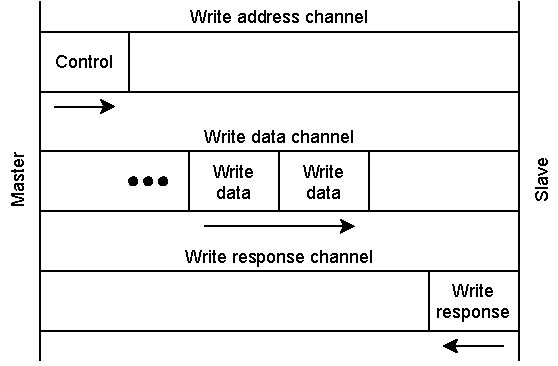
\includegraphics[width=0.45\linewidth]{WriteTrx.pdf}
  }
  \hfill
  \subfloat[Read channels.\label{fig:axi4r}]{
    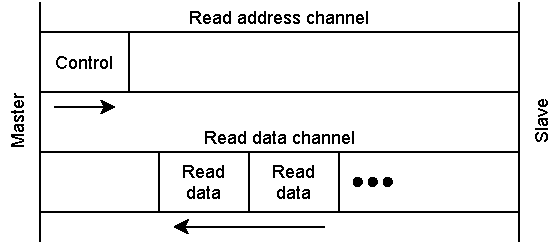
\includegraphics[width=0.45\linewidth]{ReadTrx.pdf}
  }
  \label{fig:axi4}
  \caption{An overview of the channels defined in the AXI4 standard.}
\end{figure*}

%\begin{itemize}
%  \item \textit{Write Address} for transferring transaction attributes from master to slave
%  \item \textit{Write Data} for transferring write data and strobe from master to slave
%  \item \textit{Write Response} for transferring transaction status of a writes from slave to master
%  \item \textit{Read Address} same as \textit{Write Address}, but for reads
%  \item \textit{Read Data} for transferring read data from slave to master
%\end{itemize}

Consider for example a write transaction of 16 data elements. First, the master provides transaction attributes (e.g., target address and data size) as a single transfer over the \textit{Write Address} channel, then the master transfers the 16 data elements one at a time over the \textit{Write Data} channel, and finally, the slave indicates the status of the transaction over the \textit{Write Response} channel. The \textit{Read Address} and \textit{Read Data} channels may operate independently at the same time. A full description is available in \cite{axi4standard}.

\subsubsection{Implementation}
Our implementation includes bundles defining the five different channels, abstract classes representing both master and slave entities, transaction-related classes, and of course the BFM itself; the \texttt{FunctionalMaster} class. The BFM is parameterized with a DUT that extends the slave class and provides a simple, transaction level interface to control the DUT. As such, its two most important public methods are \texttt{createWriteTrx} and \texttt{createReadTrx} which do exactly as their names indicate; create and enqueue write and read transactions. \\

Internally, the BFM makes use of ChiselTest's multithreading features to allow for (a) non-blocking calls to the aforementioned methods (i.e., one can enqueue multiple transactions without waiting for their completion) and (b) emulating the channel independence more closely. As such, when, for example, a write transaction is enqueued and no other write transactions are in-flight, the BFM spawns three new threads, one for each required channel. The threads each handle the handshaking necessary to operate the channels.

\subsubsection{A Simple Example}
Consider as an example using the BFM to test a module called \texttt{Memory}, which is now as simple as shown below. Creating a write transaction with 16 data elements (minimum burst length is 1, hence \texttt{len = 15} means a burst of 16 items) takes just one call to a method the majority of whose arguments have default values. It is equally simple to create a subsequent read transaction. Beware that due to channel independence, not waiting for a write to complete before starting to read from the same address may return incorrect results depending on the implementation of the DUT.
\begin{lstlisting}[language=scala, caption={Using the AXI4 BFM with ChiselTest}, label={lst:axitest}]
class MemoryTester extends FlatSpec with ChiselScalatestTester {
  behavior of "My Memory module"
  it should "write and read" in {
    test(new Memory()) { dut =>
      val bfm = new FunctionalMaster(dut)
      master.createWriteTrx(0, Seq.fill(16)(0x7FFFFFFF), len = 15, size = 2)
      master.createReadTrx(0, len = 15, size = 2)
    }
  }
}
\end{lstlisting}

\section{Use Case: Sorting in Hardware}

In the process of the research we implemented a use case provided by Microchip to evaluate our verification library.

\subsection{Specification}

The provided specification document describes a priority queue which can be used in real-time systems for the scheduling of deadlines by providing information about the 
next timer expiration to the host system. Sorting of the enqueued elements is conducted by applying the heap sort algorithm. Elements are structured in a so-called 
heap, which is a tree data structure. The tree needs to be balanced in order for the
timer closest to expiring to get to the top of the tree and thus to the head of the queue. This means verifying that every parent node is smaller than the connected child nodes.


The $\log_k N$ depth of the tree provides good scalability in terms of insertion and removal times when the queue size increases, 
since worst case $\log_k N-1$ swap operations need to be conducted in order to rebalance the heap. Here $k$ is the number of child elements per parent and $N$
is the number of elements in the heap. A trade-off is the varying delay connected to the rebalancing of the tree where the queue is unresponsive. If queuing
happens in bursts, a buffer could be added. Here the introduced delay from insertion request to actual appearance of the enqueued value in the heap of course needs
to be taken into account.

In order for the host system to have the ability to distinguish between multiple consecutive super cycles \hjd{What's this?} and clock cycles in a super cycle, the values inserted 
into the queue are split into the fields \textit{cyclic} and \textit{normal} priority (time out value). The removal functionality of the queue requires a reference system. A reference 
ID is therefore given together with the element at insertion, where ID generation and uniqueness are handled by the host system.

\subsection{Implementation}

The implemented priority queue is described in Chisel.
It is split into 3 modules: The \texttt{Heapifier}, responsible for the sorting, the \texttt{QueueControl}, taking care
of the general control flow in the queue and the \texttt{Memory} module which handles memory accesses and can search the memory for a specific reference 
ID.

In order for the priority queue to work efficiently, it is crucial to optimize memory accesses. Therefore a layout is proposed in the specification where all 
child elements of a certain node are stored together under one memory address. This allows single memory access fetches of all $k$ children. Since 
the root node has no siblings, it is stored alone in a register. This enables even faster access in certain scenarios which are discussed later on.

One memory row contains $k$ elements each consisting of the 3 introduced fields: \textit{cyclic} priority, \textit{normal} priority and the connected
reference ID. In the implemented 
\texttt{Memory} module, a single sequential memory is instantiated where masking is used to be able to over-write specific elements in one memory row.

There are a variety of solutions to the problem of content addressability which is required here in order to find positions of elements in the heap by providing
their reference ID. Cache-like memory relying on parallel tag comparison could be used to achieve fast and constant search times. On the other hand, the 
existing sequential memory could be searched through linearly, where $k$ reference ID's are compared in parallel until the reference ID is found.
A compromise between the two solutions could include splitting memory space over multiple instances of the latter and thus reducing worst case search time.
The priority queue is designed to be independent of the specific implementation. As a reference, the linear search is implemented.

The \texttt{Heapifier} loops from a given starting point in the tree either upwards or downwards until it hits the root or a childless node. In each iteration 
it is checked whether the parent element is smaller than its child elements and if not a swap occurs. Once the parent element and child elements of the starting 
point are fetched from memory, only the next parent or block of children respectively needs to be fetched depending on the looping direction (up/down). Thus 
only 3 cycles (1 fetch, 2 write backs) are required per swap. The state diagram of the \texttt{Heapifier} is shown in figure~\ref{fig:pq_heapifier_state}.

\begin{figure}
	\centering
	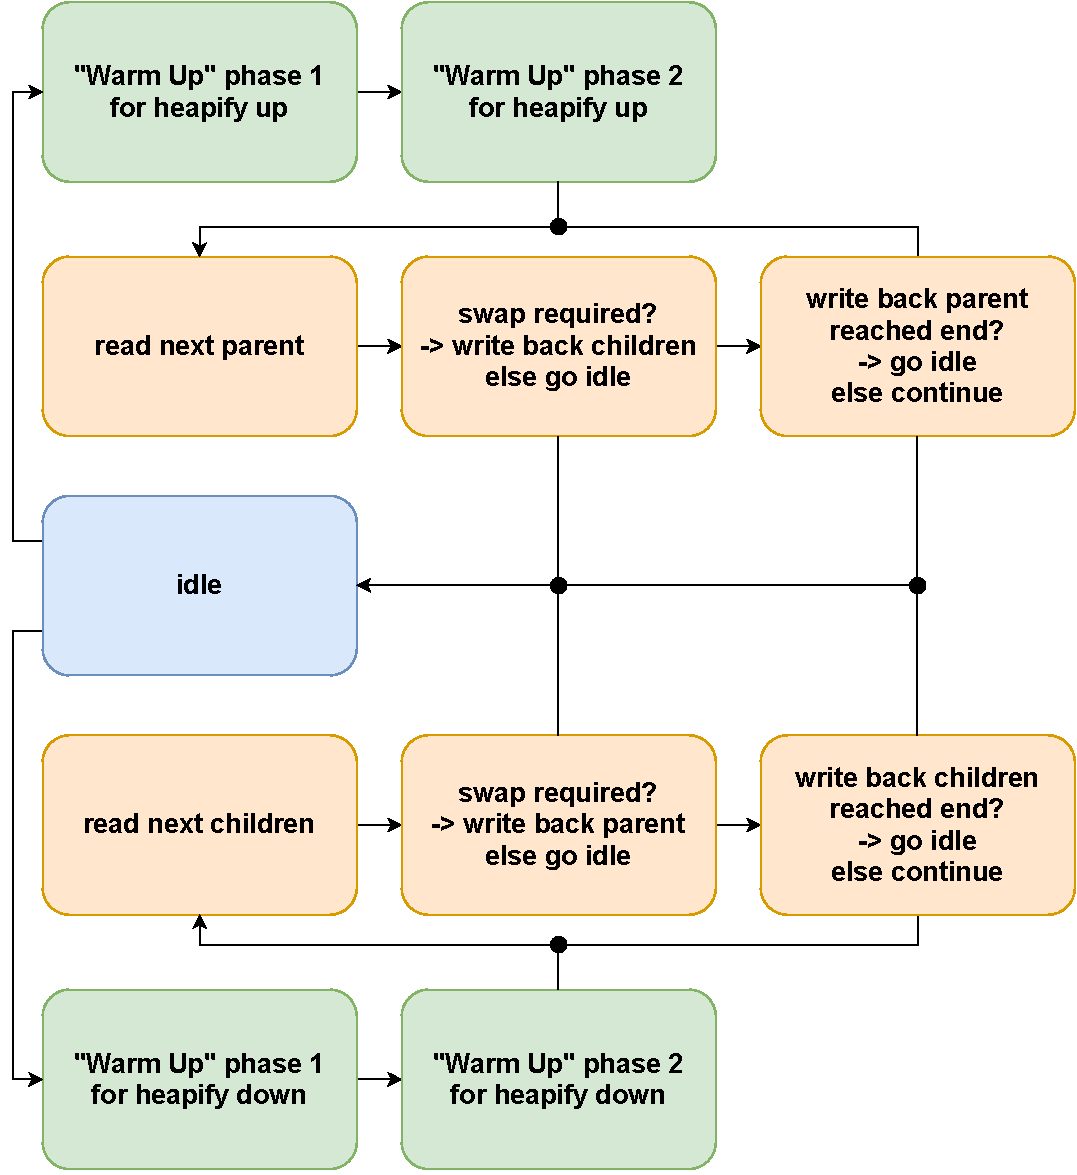
\includegraphics[width=9cm]{HeapifierStateDiagram.pdf}
	\caption{The state diagram of the \texttt{Heapifier}}
	\label{fig:pq_heapifier_state}
\end{figure}

The task of the \texttt{QueueControl} is to insert or remove elements and then signal to the \texttt{Heapfier} to balance the tree. As it can be seen in figure~\ref{fig:pq_control_state}, there are a series of special cases where insertion or removal times can be reduced for instance by taking advantage of the head element
being stored in a register. The achieved best and worst case insertion as well as removal times are presented in table~\ref{tab:pq_timings}.

\begin{figure}
	\centering
	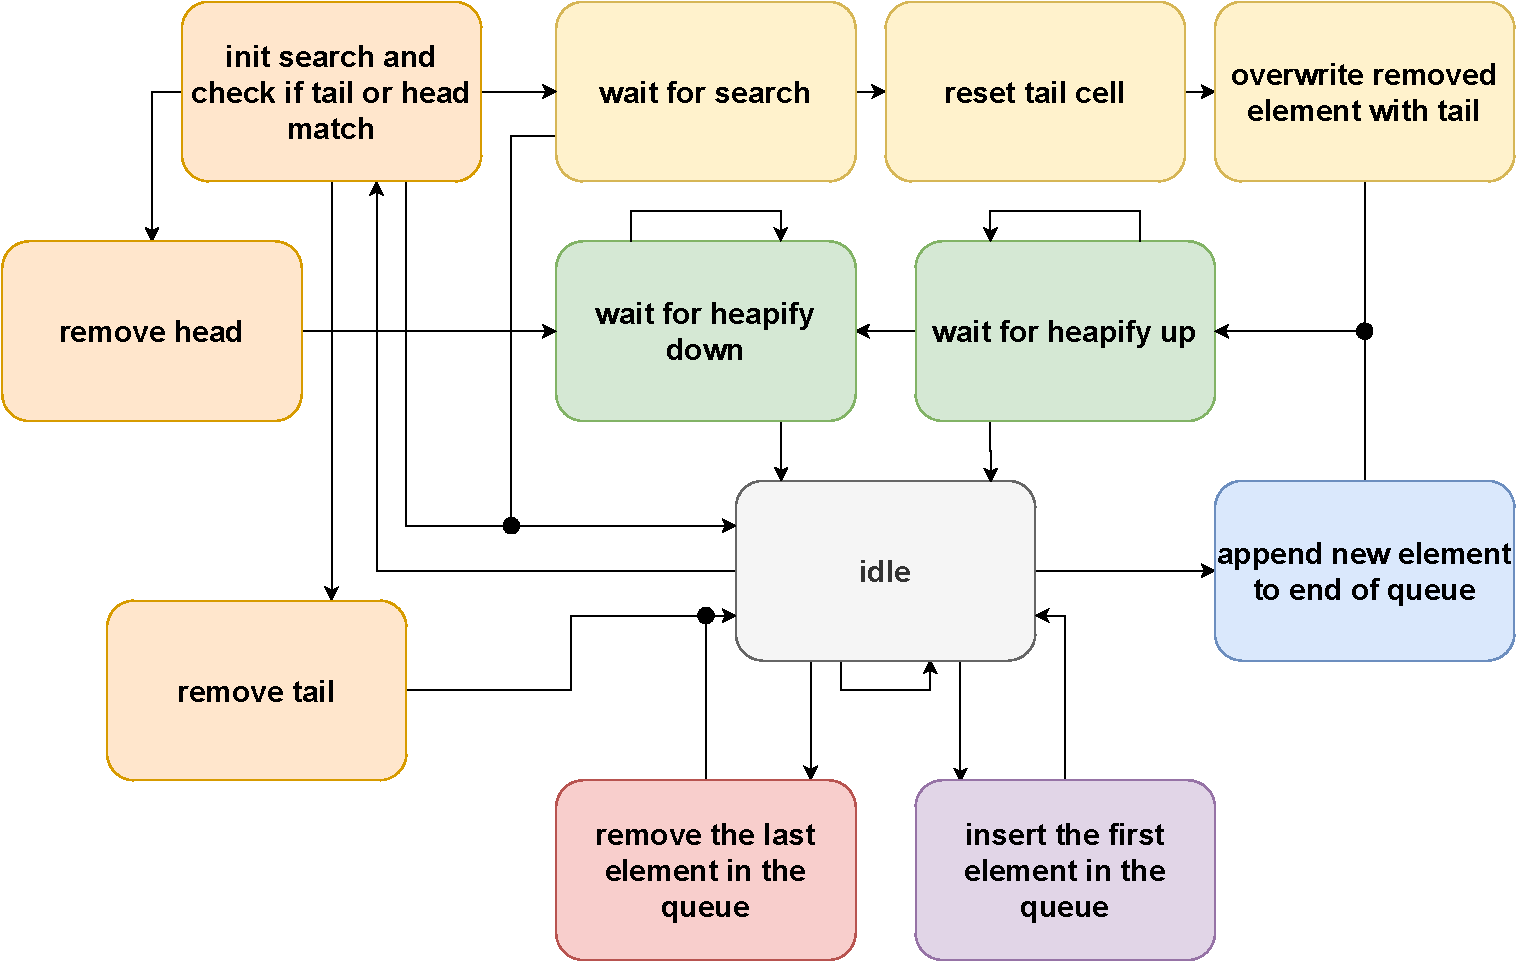
\includegraphics[width=9cm]{QueueControlStateDiagram.pdf}
	\caption{The state diagram of the \texttt{QueueControl}}
	\label{fig:pq_control_state}
\end{figure}
\begin{table}
	\centering
	\begin{tabular}{l|c}
		Head insertion & 2 cycles \\
		Normal insertion & min 7 cycles and max $5+3\cdot \mathrm{log}_k(N)$\\
		Head removal & min 8 cycles and max $6+3\cdot \mathrm{log}_k(N)$\\
		Tail removal & 3 cycles\\
    Normal removal & \begin{tabular}{c}min 12 cycles + search time\\ max $13+3\cdot \mathrm{log}_k(N)$ + search time \end{tabular} \\
    \multicolumn{2}{c}{\scriptsize{($N=$ queued elements, $k=$ number of child elements per node)}}
	\end{tabular}
	\caption{Best and worst case insertion and removal times}
	\label{tab:pq_timings}
\end{table}
\begin{table}[]
  \centering
  \begin{tabular}{l|cccc}
      Size &$k=2$&$k=4$&$k=8$&$k=16$\\\hline
      16+1 & 9.38/14.56&7.86/11.51&7.47/10.42&-\\
      32+1 & 9.9/15.15&7.96/12.29&7.34/11.22&7.54/11.00\\
      64+1 & 9.79/16.34&8.01/13.80&7.41/12.38&7.32/11.18\\
      128+1 & 9.96/17.37&8.14/14.47&7.54/13.14&7.26/11.62\\
      256+1 & 9.73/17.39&8.15/15.54&7.53/14.21&7.34/12.89
  \end{tabular}
  \label{tab:pq_simres}
  \caption{Simulated insertion/removal times.}
\end{table}

\subsection{Testing and Verification}

All modules and the fully assembled queue were tested with random stimuli in Scala by employing the \textit{ChiselTest} framework.
In order to check whether the DUT matched the specification, reference models were written for each module. Most modules 
could be modelled by a single or multiple functions. As a reference model for the whole priority queue, a class 
was written which simulates state and interaction on the operation level. In order to abstract interaction with the DUT,
wrapper classes (i.e., classes similar to BFMs) were employed. These make it easy to think on a transaction or 
operation level when writing tests.

In the test of the priority queue, purely random pokes are produced. In order to evaluate how well these pokes are spread over the spectrum 
of possible or interesting input combinations, the functional coverage feature of ChiselVerify is used. This allows to evaluate whether interesting 
or important edge cases are reached by the random input sequence. Furthermore, metrics on how many of the generated pokes actually are valid 
operations, are collected. The average insertion and removal times measured under a random test run are shown in table~\ref{tab:pq_simres}.
These numbers are dependent on access patterns and are as such only representative for the random test case used here.
%The tests can be found in the \href{https://github.com/chisel-uvm/chisel-verify/tree/master/src/test/scala/heappriorityqueue}{project repository}.

\section{Related Work}
Our current work does not find itself isolated in the Chisel verification universe. Other solutions do currently exist and we try to discuss a few of them in this section.  

\subsection{SystemVerilog for Verification}
As mentioned earlier, SystemVerilog is quite prevalent when it comes to verification. Being a mostly non-synthesisable extension of the Verilog HDL, it does contains certain constructs capable of gathering coverage information~\cite{spear2008systemverilog}, such as statement and functional coverage, in a manner similar to what we have developed. SystemVerilog can thus be used, along with the generated Verilog code, for the verification of a Chisel design. However this greatly hinders the purely Scala based workflow that our solution offers. When it comes to functional coverage, our solution offers many features that SystemVerilog does not, such as more interesting \texttt{CoverPoints} that can take temporal relations into account and generalized functional bins that work using purely user-defined hit conditions, whilst SystemVerilog only offers bins that cover value ranges or transitions. These more advanced features are possible thanks to the functional nature of Scala. 

\subsection{Universal Verification Methodology}
An other important player in the Verification world is the \textit{Universal Verification Methodology}(UVM). UVM was created a a stardardized way of writing test-benches and was mostly paired up with SystemVerilog. The interesting thing about UVM is that it allows for the creation of reusable test-benches (i.e. using the same test for multiple designs)~\cite{uvm2015}, however it is extremely verbose and even a simple test required around 1000 lines of SystemVerilog code. UVM thus requires a decent initial time-investment, but is quite reusable once it gets up and running. This method can be used to verify Chisel designs, however the fact that UVM tried to "reinvent the wheel" makes it less accessible than the simpler approach done by ChiselTest.

\subsection{Other Chisel-Specific Verification Work}
At the time of writing this, there are only a couple instances (other than the work presented in this paper) of verification work aimed specifically at Chisel. One example of this is \texttt{chisel3.formal}, which is a formal verification package containing a set of tools and helpers for formally verifying Chisel modules~\cite{chisel:formal}. The approach taken here is quite different from what we've developed. Rather than creating a set of tools that supplement the current chisel testing pipeline, \texttt{chisel3.formal} rather proposes a different way of testing, based around defining a set of formal checks that a design must pass in order to be considered as functional. These checks can, for example, look like: \texttt{past(io.out, 1) (pastIoOut => \{ assert(io.out >= pastIoOut) \})} which guarantees that the current module will never decrease its output from one cycle to the next. These formal checks can then be verified by calling the \texttt{verify(module)} function. 

This approach is similar to software contracts in Scala. The main difference between our solution and this one is that here the rules are written on a per-module basis and are thus directly linked to the Chisel code, while our solution rather focuses on checking that a suite of test-benches are testing the right things. The \texttt{chisel3.formal} package has also been extended in \texttt{kiwi-formal}~\cite{chisel:kiwi-formal} and \texttt{dank-formal}~\cite{chisel:dank-formal}, leading to multiple different versions of it, each adding their own additional formal rule templates. 

As far as we know, ChiselVerify is one of the only verification frameworks allowing for the simple use of verification functionalities, well integrated into the ChiselTest-Chisel ecosystem.

\section{Conclusion}
In this paper, we introduced ChiselVerify, an open-source solution that should increase a verification engineer's productivity by following the trend of moving towards a more high-level and software like ecosystem for hardware design. With this, we brought functional coverage, statement coverage, constraint random verification and transactional modelling to the Chisel/Scala ecosystem, thus allowing for the improvement of current engineer's efficiency and easing the way for software engineers to join the hardware verification world.

\subsection*{Source Access}

This work is in open source and hosted at GitHub: \url{https://github.com/chiselverify/chiselverify}

\subsection*{Acknowledgment}

This work has been performed as part of the
``InfinIT -- Innovationsnetv{\ae}rk for IT'', UFM case no. 1363-00036B,
``High-Level Design and Verification of Digital Systems''.

\bibliographystyle{splncs04}
\bibliography{../msbib,../chisel-uvm,../funding/ftp-chisel/testing}


\end{document}
